The main concern of the \lasii~project was to design a calibration system without \lasi~shortcomings while maintaining a high performance level in terms of precision and stability. The major improvements are summarized in Table \ref{tab:lasii_imp}.
\begin{table*}[!htpb]
 \begin{center}
\caption{Critical points of the \lasi~system and improvements in the \lasii}\label{tab:lasii_imp}
 \begin{tabular}{ll}
\hline
Critical Point & Improvement \\
\hline
Insufficient measurement of the \laser~light & Number of photodiodes increased to 10+1 \\
at each point of the optical path & \\
\hline
%Adapt the calibration system of the photodiodes & Redundant calibration scheme: \\
Cross-talk, grounding and instability problems & Redundant calibration scheme: \\
in the calibration system & Light Emitting Diode (LED) \\
of the photodiodes& and a static radioactive source \\
\hline
Insufficient light mixing of each optical set & New design of the beam expander \\
& (light to the ~400 fibers of the TileCal)  \\
& and of other mixers \\
& (\laser~head and filter wheel outputs) \\
\hline
 & Optics box in an horizontal position\\
Optics box in a vertical orientation& (minimize dust deposits on optics \\
& and ease maintenance) \\
\hline
Saturation of the photodiode electronics & Increased dynamic range (13 bits-ADC) \\
\hline
Electronics shortcomings  & New card including all functionalities \\
(LASTROD memory, LHC clock) & \\
\hline
\end{tabular}
%\caption{Critical points of the \lasi~system and improvements in the \lasii}\label{tab:lasii_imp}
\end{center}
\end{table*}
\par
A better estimation of the \laser~light injected in the system is possible with an increase of the number of photodiodes. In that case, the implementation of a system using a moving radioactive source to monitor the photodiodes (as for \lasi) is difficult. We thus moved to a system comprised of a Light Emitting Diode (LED) and a static radioactive source. The LED signal is injected in the ten photodiodes dedicated to the measurement of the \laser~light and in a reference photodiode monitored with a static radioactive source. 
\par
The optical path, that is the path followed by the \laser~light, is a critical point of the \lasii~system. A lot of efforts has been devoted to ensure good stability and uniformity of the light transmitted to the PMTs of the TileCal. Two aspects have been worked on: the layout of optical elements and the light mixers. \par
The optics box is set in an horizontal position to minimize the dust accretion on optical parts and to ease interventions and maintenance. \par
The goal of light mixers is to expand the \laser~beam diameter from about 700 \mum~(original size) up to a few centimeters (size of the bundle of 400 fibers). As described below, they have been redesigned to optimize homogeneity of the light distribution, minimize beam pointing effects and  guarantee the stability of the light transmitted.
\par
Electronics has been redesigned to correct for shortcomings seen with the \lasi~system. The dynamic range of the photodiode preamplifiers has been extended to avoid saturation effects for higher \laser~intensities. The boards used to drive the \lasi~system (LASTROD, LILAS, SLAMA,...) are now gathered on a single card, LASer Control Acquisition Readout (\lascar), to improve the communication between the boards (LASCAR has only one FPGA).
\par
A scheme of the \lasii~system is given in Figure \ref{fig:laserscheme} and is comprised of the following parts:
\begin{figure}[htbp]
\centering
%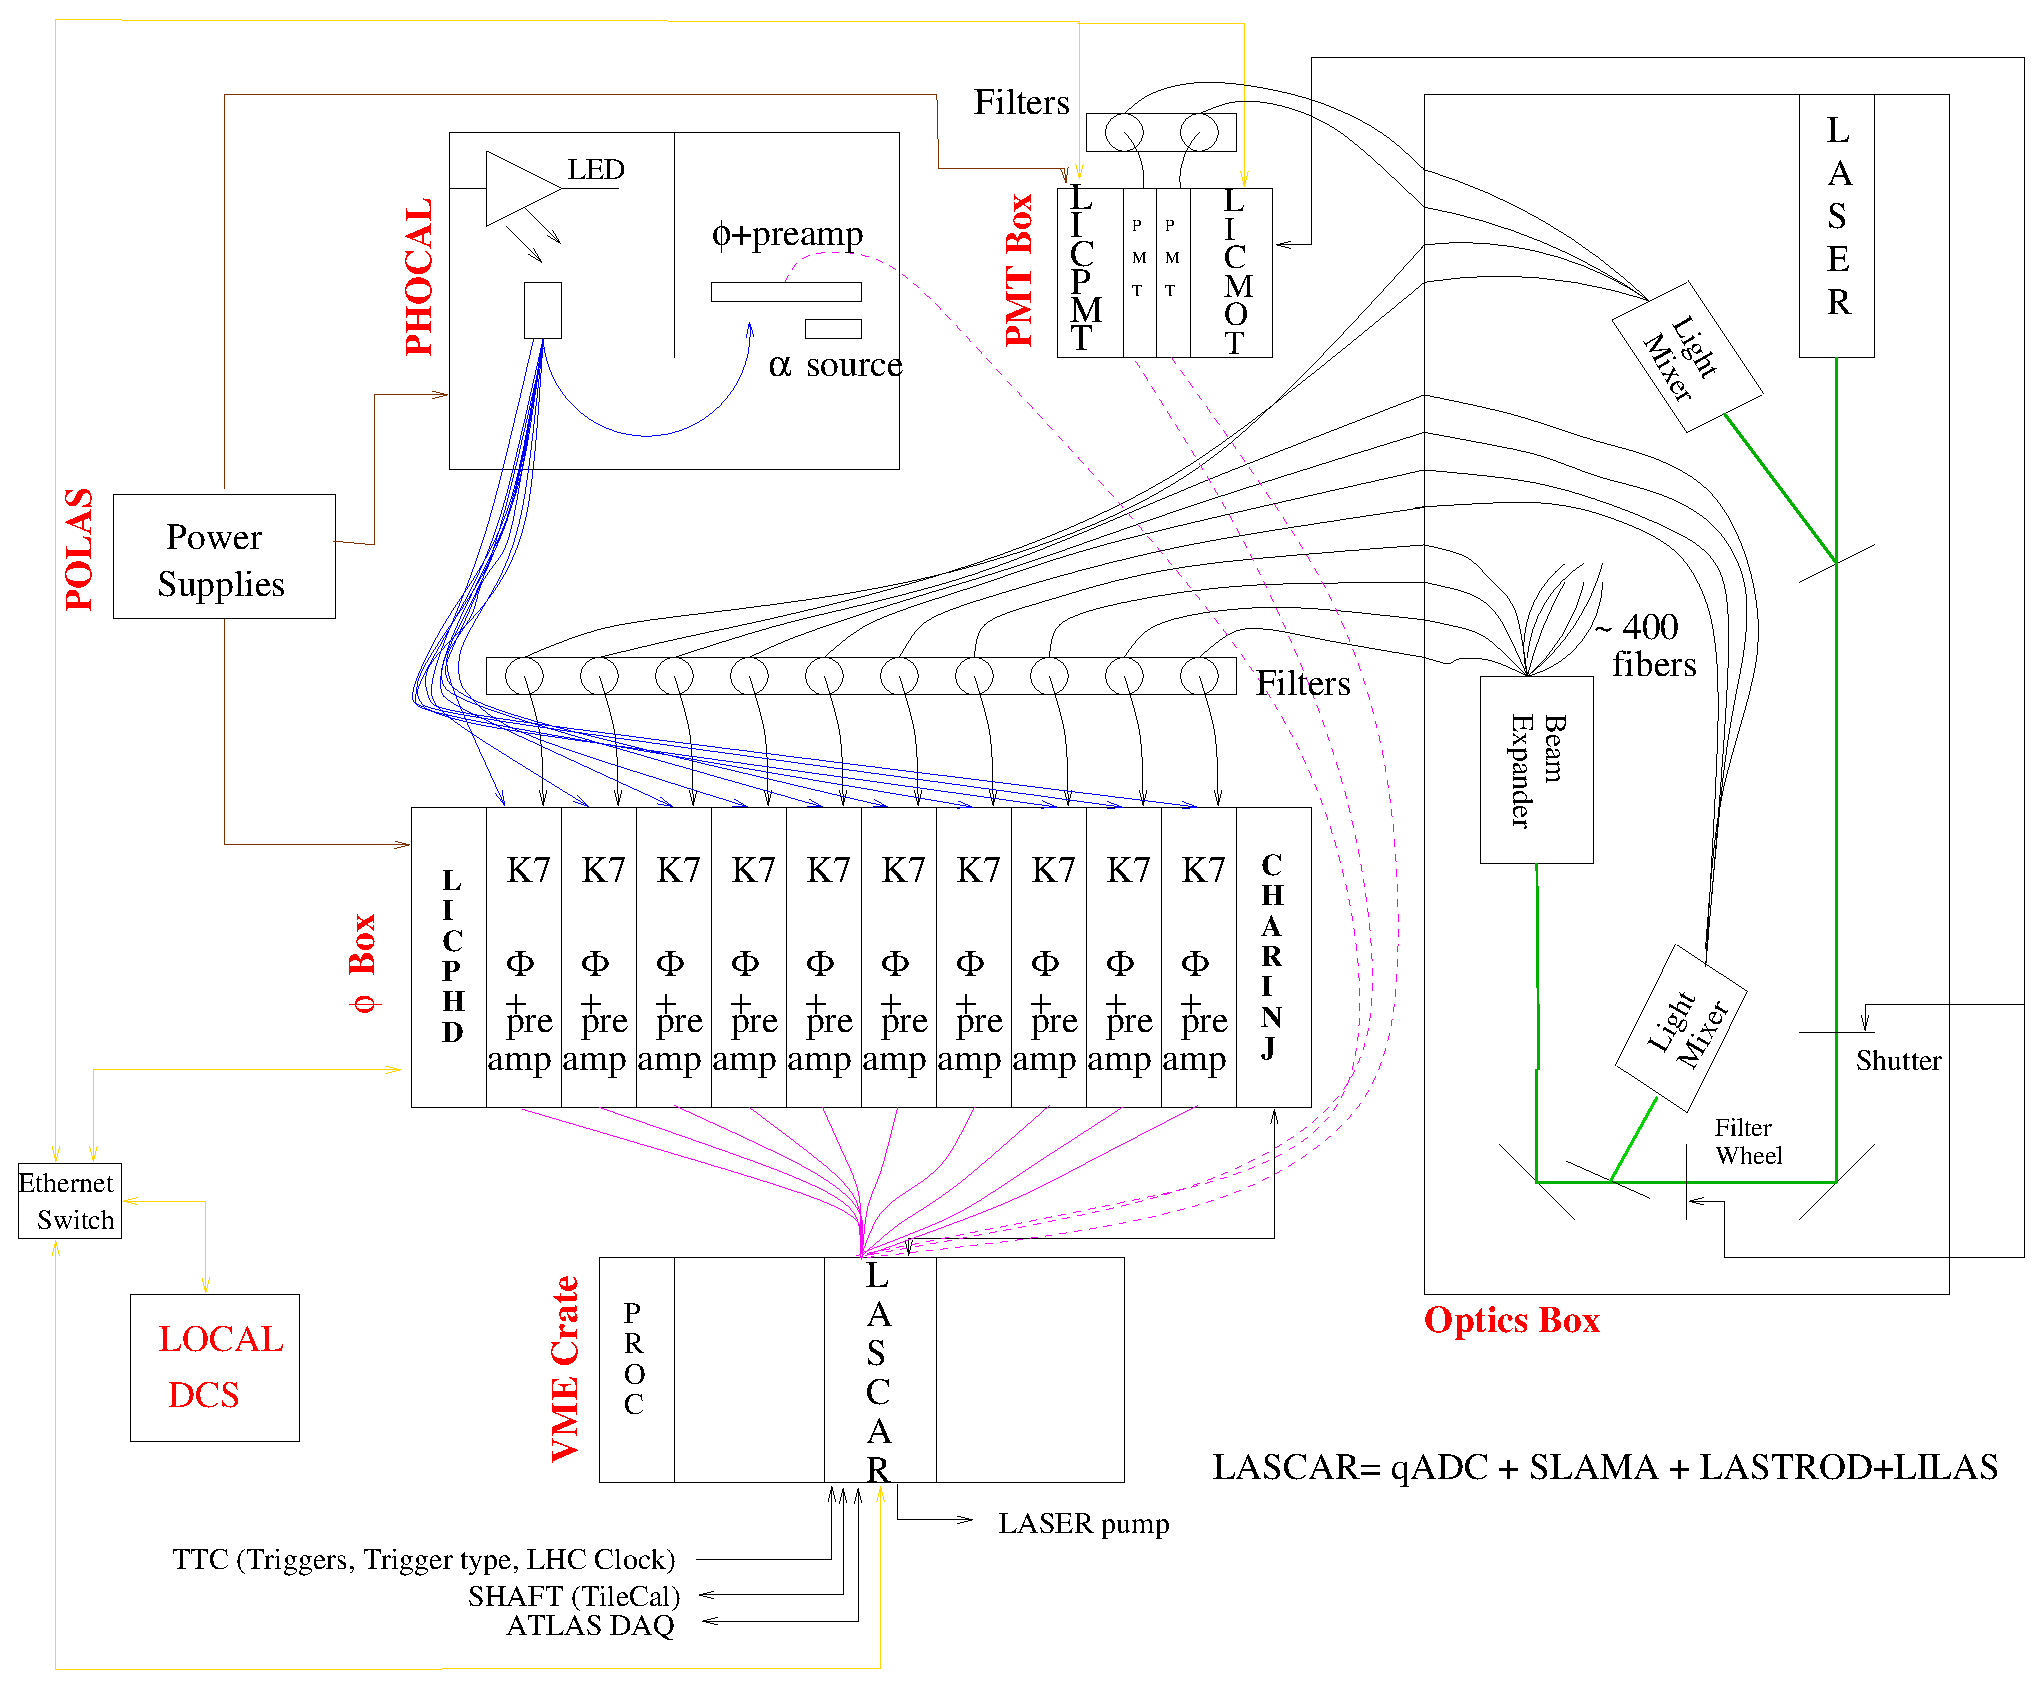
\includegraphics[width=11cm,height=11cm]{figures/LaserII_latest_latest.eps}
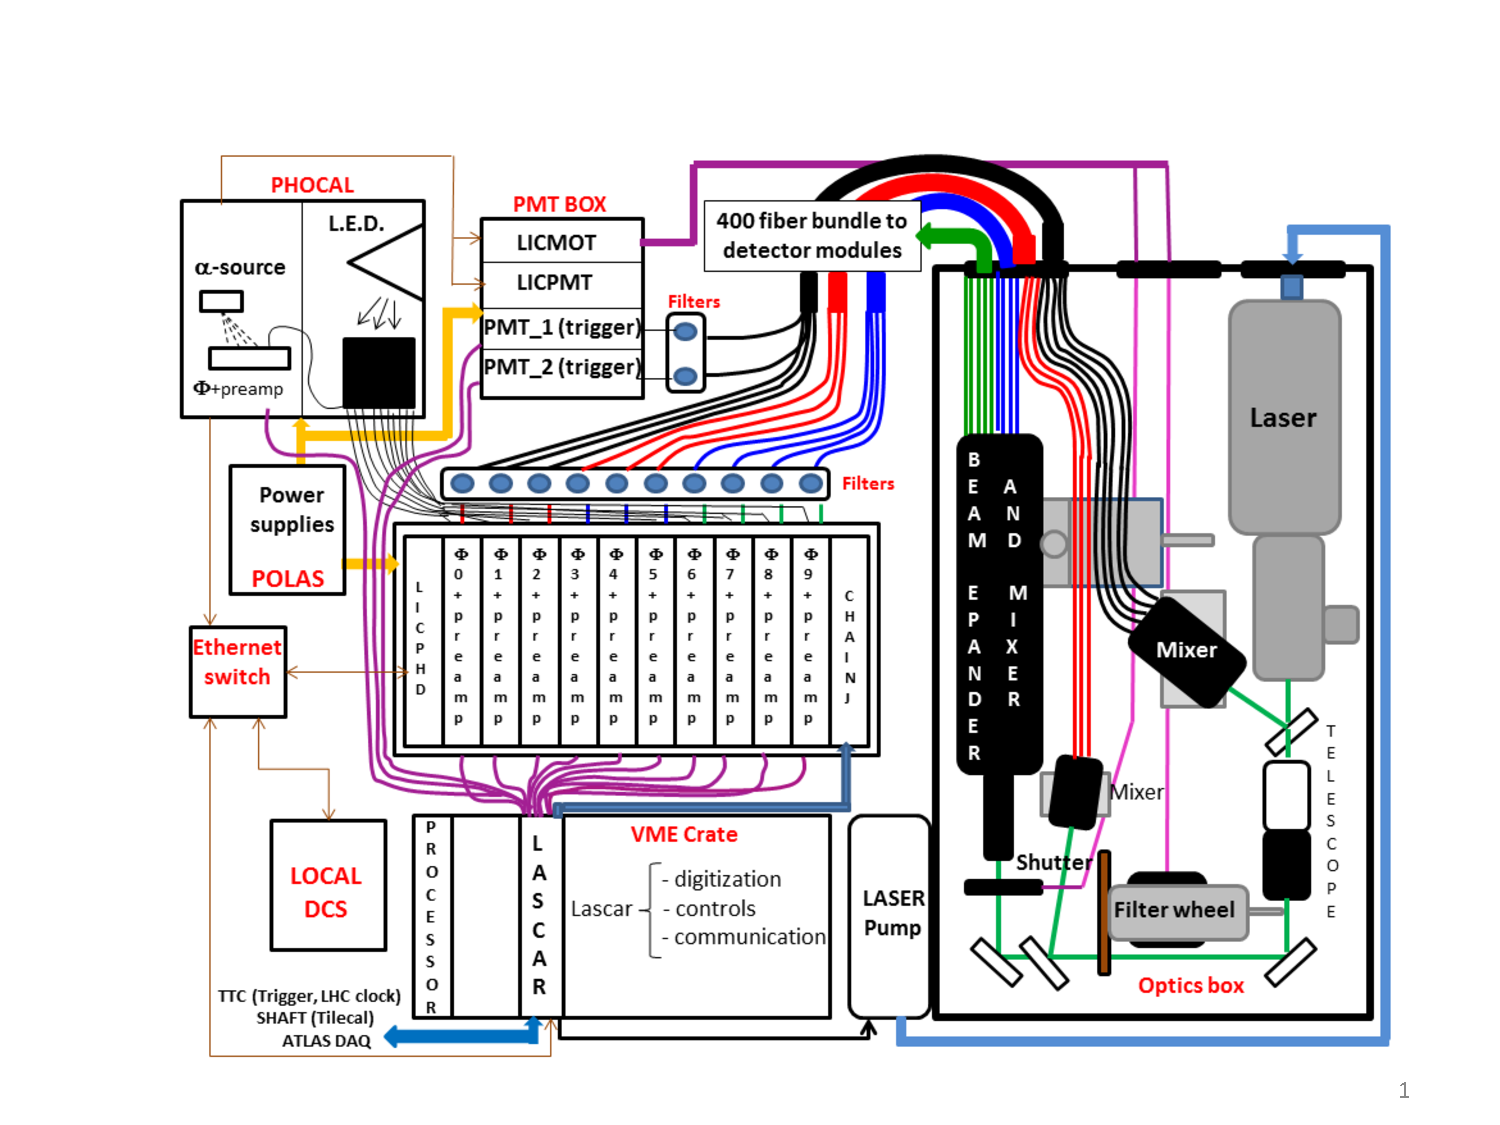
\includegraphics[width=15cm]{figures/Laser_II_layout.pdf}
\caption{Scheme of the \lasii~system}\label{fig:laserscheme}
\end{figure}
\begin{itemize}
\item Optics box: at the output of the laser head, the beam is divided into two parts: one 
is sent back to a light mixer that dispatches the light to seven optics fibers (three are connected to photodiodes) while the other is transmitted through a beam expander ($\times$2.5) and a 45$^{o}$ mirror to a filter wheel. At the output of the filter wheel, the beam is splitted with one part sent to a light mixer (of the same kind as the first one, connected to three photodiodes) and the other part is sent to a beam expander which magnifies and dispatches the input light to a bundle of about 400 fibers. Four fibers are connected to photodiodes while all others transmit the light to the TileCal modules.

%at the output of the \laser~head, the beam is transmitted through a beam expander (x2.5) and divided in two parts: one is sent to a light mixer that dispatches the light to seven optics fibers (3 are connected to photodiodes) while the other is reflected by a miror and transmitted to a filter wheel. At the output of the filter wheel, the beam is splitted with one part sent to a light mixer (of the same kind as the first one, connected to three photodiodes) and the other part is sent to a beam expander which magnifies and dispatches the input light to a bundle of about 400 fibers. 4 fibers are connected to photodiodes while all others transmit the light to the modules of the TileCal.

\item Photodiode box: this box houses ten modules dubbed cassettes. Each cassette contains a photodiode (and its amplifier) that receives light from the optics box (\laser~beam) or from the PHOtodiode CALibration (\phocal) module (LED signal). This box also contains two electronic boards, LICORNE\footnote{LICORNE is the Laser Independent COntrol Remote Network.} Photodiode (\licphd), an electronic board used to drive the photodiode box,~and a charge injection splitter (\charinjsplit), a module dispatching a charge that aims at monitoring the stability of the electronics,

\item \phocal~is an internal calibration system setup to monitor the stability of the ten photodiodes located in the photodiode box. It is composed of a LED emitting a signal in a light mixer that transmit the light to a set of eleven optics fibers, with ten connected to the photodiode box, and one coupled to a reference photodiode. 
The stability of the ten photodiodes is performed by monitoring the ratio of the LED signal seen by these photodiodes to the magnitude measured by the reference photodiode. The stability of the reference photodiode is estimated with a static radioactive source,

\item PMT box: two PhotoMultiplier Tubes (PMTs) are used to trigger the \lasii~acquisition when the \laser~is flashing. The PMT box also contains two electronic cards to drive the PMT box (\licpmt)~and the filter wheel (\licmot),

\item Optical filters are used to attenuate the \laser~signal transmitted to the photodiodes and the PMTs,

\item VME crate: two boards located in the VME crate are used to drive the \lasii~system: a VME Single Board Computer (SBC); \lascar, that incorporates on one mezzanine a charge analog-to-digital converter (qADC), as well as LILAS, and HOLA card on another mezzanine. \lascar~also includes the TTCrx chip,

\item POwer LASer (\polas): power supplies of the \lasii~system. \polas~provides low voltages (+5V, -5V, $\pm$15V,+12 V, +24 V) to electronic boards,

\item Local DCS: a PC is used to collect slow-control information (such as temperatures, position of the filter wheel,...) from LICORNE Motor (\licmot), Licorne PMT (\licpmt), \licphd~and \lascar~cards through ethernet connections.


\end{itemize}